% ===============================
%          Chapter 1B.5
%        Atherosclerosis
%     Created by Michael Tang
%           2025.01.13
% ===============================

\subsubsection{1B.5 Atherosclerosis}
\paragraph{Overview}
\begin{itemize}
    \item \underline{Cardiovascular diseases} (CVDs 心血管病) are the leading cause of death globally, responsible for 31\% of all
    global deaths (according to WHO data, 2017).
    \item Many CVDs are associated with \underline{atherosclerosis} (动脉粥样硬化), a condition where \underline{plaques} (斑块)
    build up inside arteries.
\end{itemize}

\paragraph{Atherosclerosis}
\begin{itemize}
    \item \textbf{Definition:} A desease where plaques (fatty deposits) from in arteries, narrowing the lumen and reducing blood
    flow.
    \item \textbf{Development:}
    \begin{itemize}
        \item \textbf{Step 1:} Damage to the \underline{endothelium} (内皮 e.g., due to high blood pressure or smoking).
        \item \textbf{Step 2:} \underline{Inflammatory response} (炎症反应); white blood cells migrate to the area.
        \item \textbf{Step 3:} \underline{Accumulation} (积累) of \underline{cholesterol} (胆固醇), forming a \underline{fatty
        deposit} (atheroma 脂肪沉积).
        \item \textbf{Step 4:} Calcium salts and fibrous tissue build up around the atheroma, forming a hardened plaque.
    \end{itemize}
    \item \textbf{Effects:}
    \begin{itemize}
        \item Narrowed arteries increase blood pressure.
        \item Increased risk of blood clots (\underline{thrombosis} 血栓形成) at the site of plaques.
    \end{itemize}
    \begin{figure}[H]
        \centering
        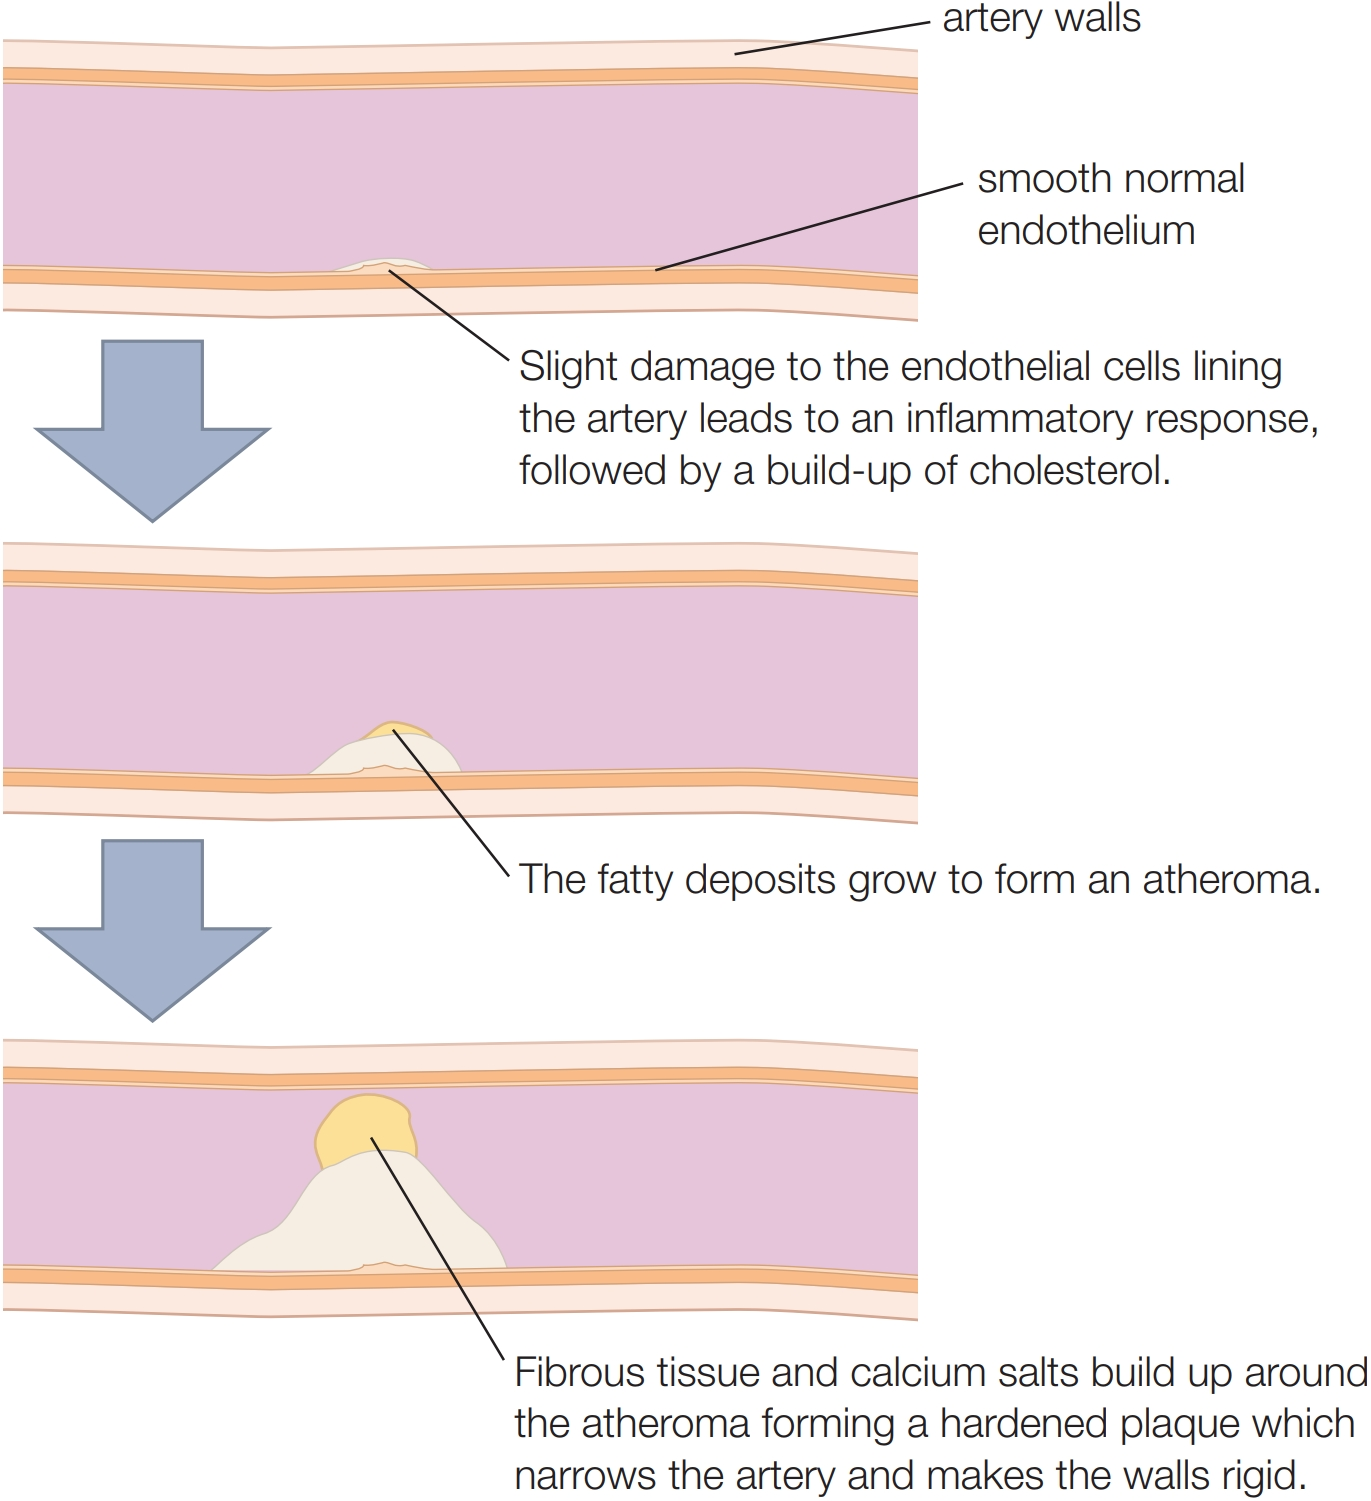
\includegraphics[scale=0.18]{Biology/1B/Images/1B-5-1.png}
        \caption{The development of atherosclerosis.}
    \end{figure}
\end{itemize}

\paragraph{Health Impacts of Atherosclerosis}
\begin{itemize}
    \item[1.] \textbf{\underline{Aneurysms} (动脉瘤):}
    \begin{itemize}
        \item Weakening of arterial walls due to plaque formation.
        \item The artery may \underline{bulge} (凸出) and \underline{rupture} (破裂), causing internal bleeding.
        \item Common in the aorta or brain arteries.
    \end{itemize}
    \item[2.] \textbf{\underline{Rised Blood Pressure} (高血压):}
    \begin{itemize}
        \item Narrowed arteries force the heart to pump harder.
        \item High blood pressure damages organs like the \underline{kidneys} (肾脏), eyes, and brain.
    \end{itemize}
    \item[3.] \textbf{Heart Diseases:}
    \begin{itemize}
        \item \textbf{\underline{Angina} (心绞痛):}
        \begin{itemize}
            \item Reduced blood flow to the heart muscle due to narrowed \underline{coronary arteries} (冠状动脉).
            \item Symptoms include chest pain, especially during exercise.
        \end{itemize}
        \item \textbf{\underline{Myocardial Infarction} (心肌梗死 Heart Attack):}
        \begin{itemize}
            \item Complete blockage of a coronary artery.
            \item Starves part of the heart muscle of oxygen, causing tissue death.
            \item Severity depends on the location and \underline{extent} (程度) of blockage.
        \end{itemize}
        \begin{figure}[H]
            \centering
            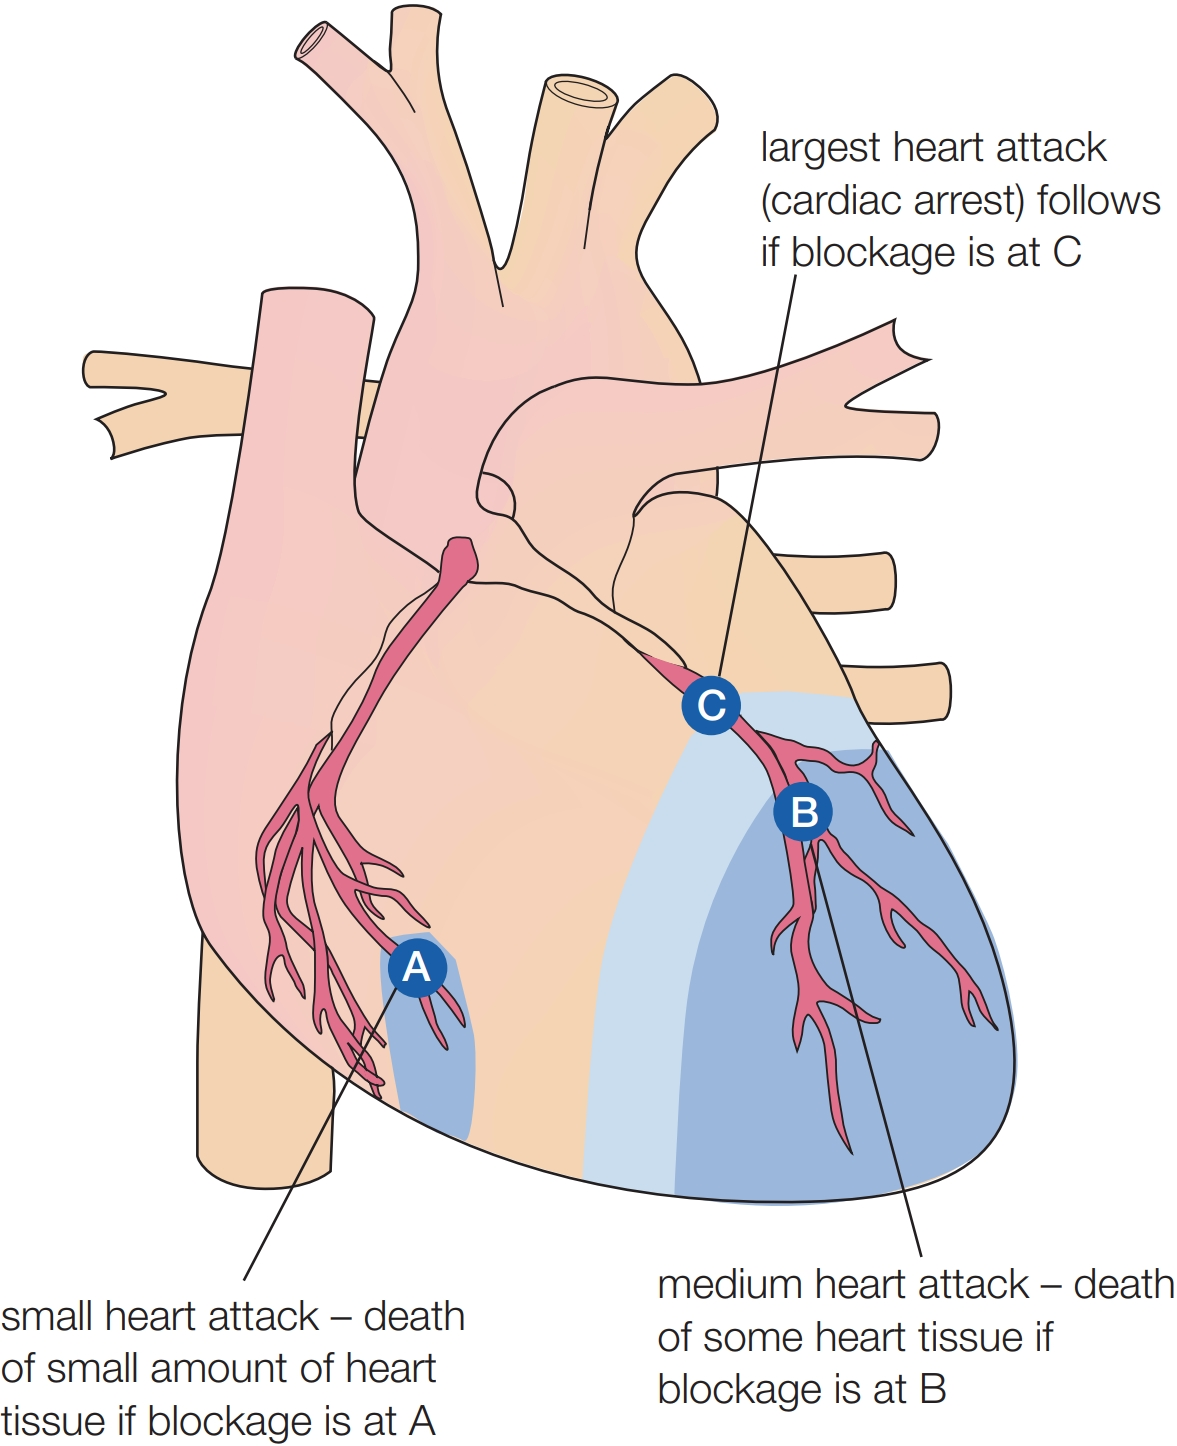
\includegraphics[scale=0.18]{Biology/1B/Images/1B-5-2.png}
            \caption{The size and severity of a heart attack is closely related to the position of the blockage in the coronary
            artery.}
        \end{figure}
    \end{itemize}
    \item[4.] \textbf{\underline{Stroke} (中风):}
    \begin{itemize}
        \item Disruption of blood supply to the brain due to a clot or \underline{hemorrhage} (出血).
        \item Symptoms include \underline{dizziness} (头晕), \underline{slurred speech} (口齿不清), and \underline{paralysis} (瘫痪).
        \item Quick treatment with \underline{clot-busting drugs} (溶栓药) increases survival chances.
    \end{itemize}
\end{itemize}

\paragraph{Prevention and Treatment}
\begin{itemize}
    \item \textbf{Prevention:}
    \begin{itemize}
        \item Regular exercise.
        \item Healthy diet low in saturated fats.
        \item Avoiding smoking and managing blood pressure.
    \end{itemize}
    \item \textbf{Treatment:}
    \begin{itemize}
        \item \textbf{Medication:} E.g., Statins (降脂药, lower cholesterol levels), \underline{antihypertensives} (降压药).
        \item \textbf{Surgery:} E.g., \underline{angioplasty} (血管成形术) to widen arteries, \underline{bypass surgery} (搭桥手术),
        \underline{stent insertion} (支架植入).
    \end{itemize}
\end{itemize}